\documentclass[11pt,letterpaper,landscape]{article}
\usepackage[margin=.75in]{geometry}
\usepackage[T1]{fontenc}
\usepackage{lmodern,microtype,amsmath,booktabs,graphicx,natbib,xurl,hyperref}
\hypersetup{colorlinks=true,linkcolor=blue,urlcolor=blue,citecolor=blue}
\setlength{\parindent}{0pt}\setlength{\parskip}{.5em}
\providecommand{\reportbuilddatetime}{unknown}
\input{report-build-info.tex}
\input{report-values.tex}
\title{MDS initialization and neighborhood sensitivity\\on five sampled saddle surfaces}
\author{\small Source: \path{~/current_projects/grip/papers/grip-software-paper/reproducibility/experiments/mds-initializer-sensitivity/report.tex}}
\date{Build \reportbuilddatetime}
\makeatletter
\renewcommand{\maketitle}{\begin{center}{\Large\@title\par}\vspace{.6em}{\@author\par}\vspace{.4em}{\@date\par}\end{center}\vspace{.3em}}
\makeatother
\begin{document}
\maketitle
\section*{Question and main findings}
Does the manuscript's edge-KK path-fidelity result depend on classical scaling
as its initializer, and how sensitive is it to the symmetric $k$-nearest-neighbor
graph? We compare classical MDS and metric stress MDS, each before and after
edge-KK, on the same five existing samples. The generating coordinates provide
a fifth control. These are finite, exploratory comparisons, not a theorem about
all MDS or edge-KK solutions.

\input{report-findings.tex}

\section*{What was held fixed}
Each sample contains 1,000 area-uniform points on
$z=0.8(x^2-y^2)$ over $[-1,1]^2$. Graphs use exact ambient nearest neighbors,
symmetric union, ambient chord edge lengths, no pruning, and the original
component-MST repair rule. The selected values are $71,70,67,72,73$.
For each cloud, the frozen neighborhood choices are $32$, $k^\star-5$,
$k^\star$, $k^\star+5$, and $80$. No embedding outcome was used to choose them.
The saved 1\%-of-minimum graph/reference-error plateaus are respectively
71--72, 64--71, 65--68, 70--73, and 65--73. The $\pm5$ choices probe more broadly
than these narrow plateaus.

\textbf{The MDS inputs here are graph shortest-path distances.}
The numerical smooth-surface geodesics are independent evaluation references.
This matches the manuscript's $X\to G\to Z$ workflow. It is distinct from the
future experiment that feeds smooth-geodesic distances directly into a graph
construction and studies increasing paraboloid/saddle radius.

\clearpage
\section*{Methods and score definitions}
Classical scaling uses \texttt{grip::classical.mds()}. Stress MDS uses
\texttt{grip::metric.mds()}, with \texttt{smacof::mds(type="ratio")} as its
majorization backend; ratio disparities preserve dissimilarity ratios, with
internal target normalization \citep{mair2022}. The grip adapter restores the
raw-stress-optimal coordinate scale in the original input units. Each graph
receives a classical start and five Gaussian starts, each with a 1,000-iteration
cap and tolerance $10^{-8}$. The least achieved raw stress selects the result.
Random configurations are paired across $k$ within each cloud. Neither multiple
starts nor the stopping tolerance establishes global optimality.

Both edge-KK branches use the original density-to-uniform continuation
$(0,.25,.5,.75,1)$, 200 steps per stage, profiled target scale, and zero
edge-length stabilizer. At selected graphs, separate checks continue the
selected MDS solution for 2,000 iterations at tolerance $10^{-10}$ and each
edge-KK solution for 1,000 uniform-stiffness steps. They do not replace the
primary fits or alter their initialization.

Write $d$ for input target lengths and $y$ for observed lengths. The fitted target
multiplier is $a=y^\top d/(d^\top d)$. Edge and fixed-path errors are
$\|y-ad\|/\|ad\|$, with separately fitted scales. Chord profiled Stress-1 is
$\|y-ad\|/\|y\|$. Raw chord stress is $\|y-d\|^2$ at returned coordinate scale.
Its target-normalized RMSE and literal unprofiled Stress-1 are also saved.
With free coordinate scale, the minimum raw stress divided by $\|d\|^2$ equals
squared profiled Stress-1; this identity is independently checked.

All 499,500 unordered pairs use a retained input-graph route, fixed across
layouts on each graph. No embedded shortest paths are recomputed. For $X\to G$
error, strict graph distances are compared directly with the same 119,744
numerical surface-reference pairs per cloud. For $X\to Z$ path error, embedded
path lengths are divided by the edge-fitted scale before that comparison;
no scale is fitted to the surface reference.

Coordinate error uses known row correspondence and divides alignment RMSE by
the original RMS radius. Rigid alignment permits rotation/reflection and
translation; similarity alignment also permits uniform scaling. Surface RMS
averages the two directional mean squared closest-triangle distances after
coordinate alignment. Each embedded mesh uses original parameter-space Delaunay
connectivity; the reference subdivides those triangles twice and lifts them
onto the saddle. There are 8,000 area-uniform samples per direction. The original
mesh is a nonzero discretization control. Surface Monte Carlo SE describes
sampling error only; this statistic does not certify absence of folds.

\section*{Numerical input and validation scope}
The retained-path preparation can contain tiny directional distance differences
from its near-tie rule. A preliminary fit exposed an asymmetry of about
$2.67\times10^{-8}$, which the MDS validator correctly rejected. All final fits
therefore use the saved strict graph-distance matrices, symmetrized only at
floating-point scale, for both MDS algorithms. Retained route lengths continue
to define path diagnostics. The earlier partial run is excluded. No symmetry
validation was relaxed. Historical classical distances and scores are checked
to $10^{-7}$; independent path sums and common package scores are checked more
tightly. The saved numerical smooth-reference validation is reused and is not
a certified all-pairs accuracy bound.

\clearpage
\section*{Selected-graph comparison}
\begin{center}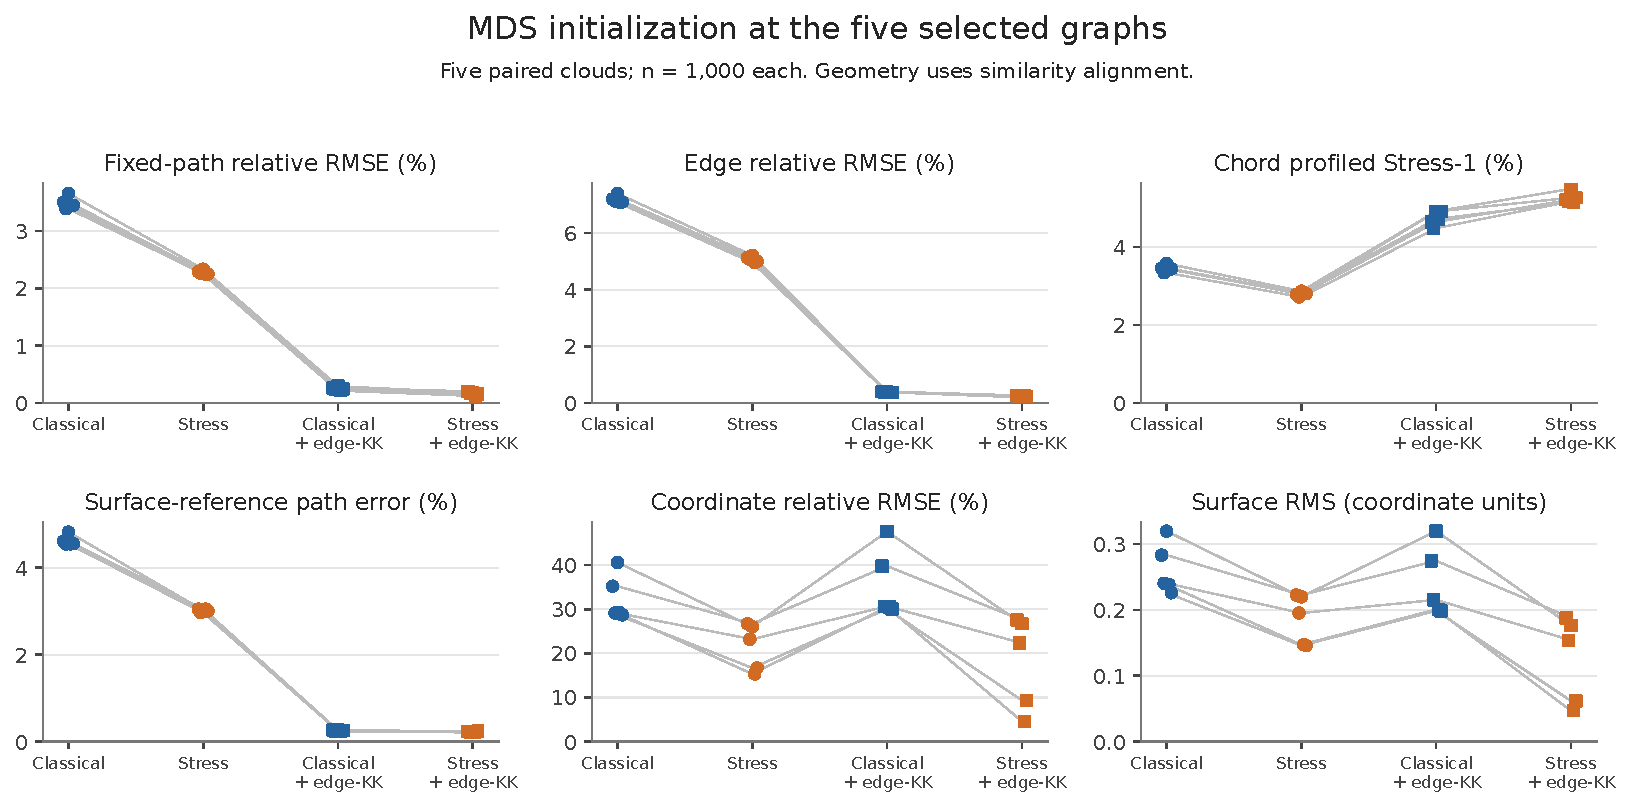
\includegraphics[width=.95\linewidth]{figures/selected-comparison.pdf}\end{center}
\small Five dots per method represent the five samples; gray lines connect the
same sample. All distance scores are percentages except surface RMS, which is
in coordinate units. Geometry uses similarity alignment. The original control
has effectively zero edge/path/coordinate error; its surface discrepancy is
nonzero because a piecewise-linear sample mesh approximates the curved reference.
The table reports medians across the five clouds.
\normalsize
\input{report-selected-table.tex}

\clearpage
\section*{Sensitivity of distance fidelity to the graph}
\begin{center}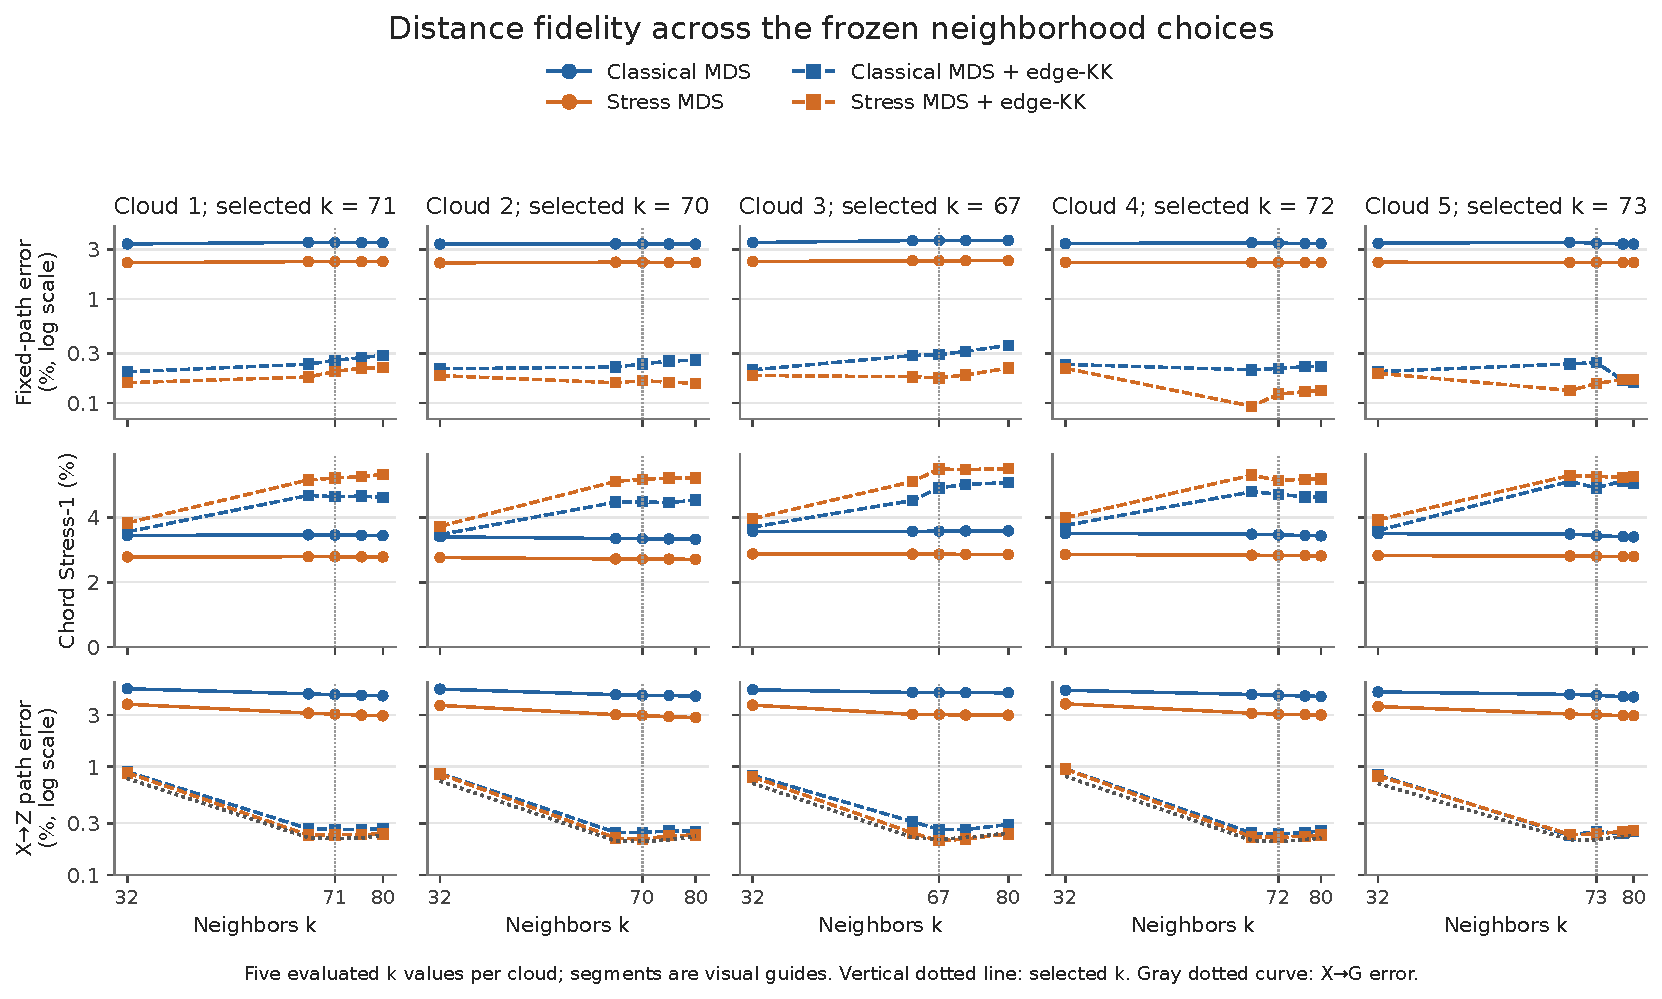
\includegraphics[width=.99\linewidth,height=.76\textheight,keepaspectratio]{figures/k-distance-sensitivity.pdf}\end{center}
\small All four candidates are paired within each cloud and graph. Path-error axes use logarithmic scales. The vertical
dotted line marks the originally selected $k$. The gray dotted curve in the
bottom row is $X\to G$ error. Segments connect evaluated settings and do not
claim behavior at every intermediate integer. Low graph-to-layout path error
cannot remove error already introduced by graph construction.\normalsize

\clearpage
\section*{Sensitivity of geometric agreement to the graph}
\begin{center}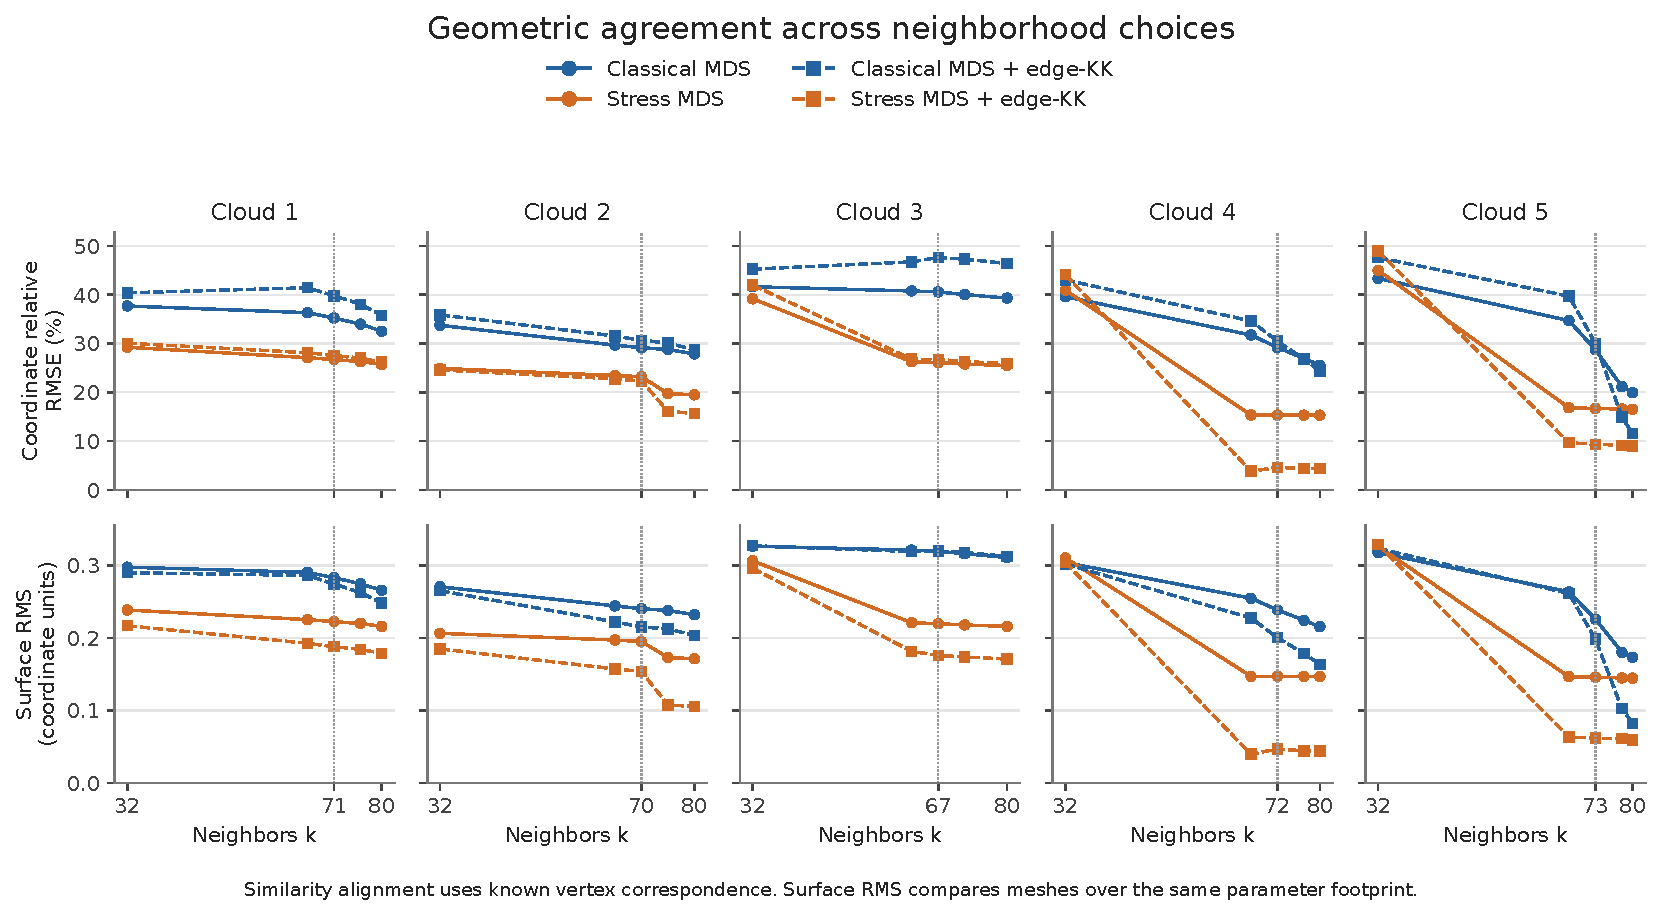
\includegraphics[width=.99\linewidth]{figures/k-geometry-sensitivity.pdf}\end{center}
\small Both rows use similarity alignment with known correspondence. The surface
statistic evaluates the same parameter footprint and mesh connectivity for every
candidate. It is an agreement diagnostic, not an injectivity or topology test.
Changes in the selected local MDS solution can contribute to irregular behavior
across $k$; the figure does not isolate graph effects from optimizer basin changes.
\normalsize

\clearpage
\section*{Optimizer and budget sensitivity}
\begin{center}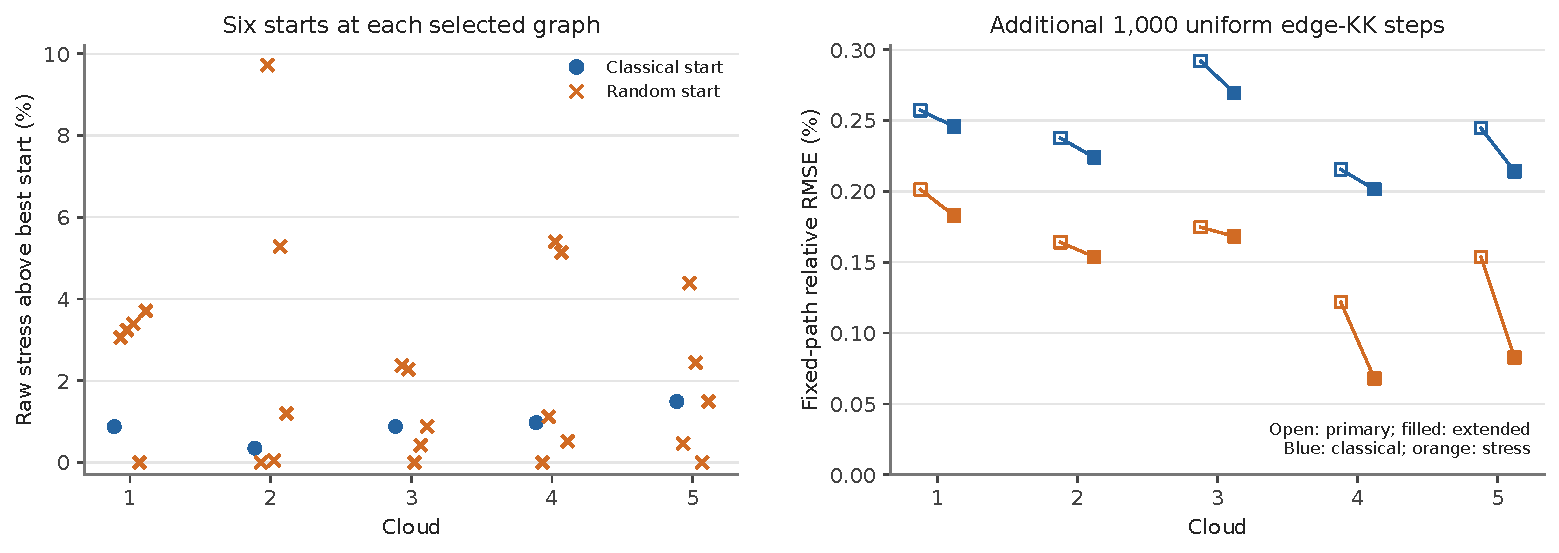
\includegraphics[width=.96\linewidth]{figures/optimizer-sensitivity.pdf}\end{center}
\input{report-optimizer.tex}
\section*{Interpretation for the software manuscript}
The graph-sensitivity result belongs in the paper because it tests a practical
choice that the current workflow asks the user to make. A concise main-text
comparison should name classical scaling and raw-stress MDS explicitly, report
both the path benefit and chord tradeoff, and show that graph/reference fidelity
is a separate requirement. The complete starts, graph diagnostics, coordinate
and surface checks, and additional-budget fits fit naturally in supplementary
reproducibility material.

These experiments do not establish recovery of the generating saddle, a planar
or tree limit, or robustness under increasing surface radius or sample size.
They also do not determine a universally best $k$. The wider radius study remains
a separate phase. The current manuscript and its original scientific caches
have not been replaced by this experiment.

\clearpage
\section*{A fixed visual example}
\begin{center}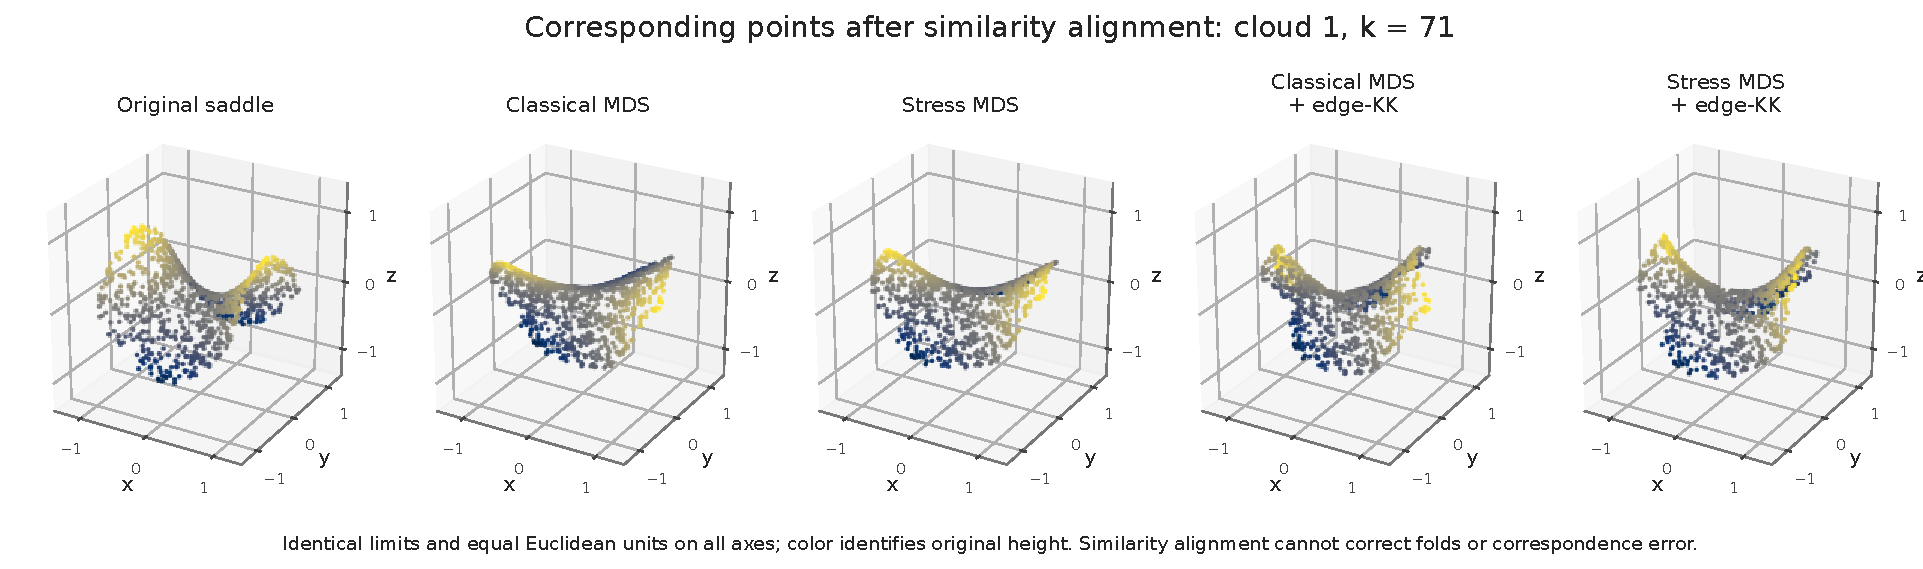
\includegraphics[width=\linewidth]{figures/selected-shapes.pdf}\end{center}
Cloud 1 is shown by a fixed first-cloud rule. All panels use the same limits and
equal Euclidean units on the three axes after similarity alignment. Color tracks
the original height of the same points. No anisotropic display rescaling is used.
The quantitative comparisons across all clouds are the basis for conclusions;
this single picture is an illustration.

\section*{Reproducibility}
The adjacent \texttt{README.md} defines the full protocol and commands.
\texttt{summary/} contains graph selection, all primary scores, 150 start records,
additional-budget scores, coordinate/surface diagnostics, timings, optimizer
status, source/input hashes, and validation. \texttt{coordinates.csv.gz} supports
figure reconstruction without optimization. Full fit and path checkpoints live
in the manuscript build tree; regenerating figures and this report uses only
tracked summaries. No computation depends on private agent notes.

\bibliographystyle{plainnat}\bibliography{references}
\end{document}
